\paragraph{Bereitstellung der Datenbank}
=> MongoDB 
=> WiredTiger Engine, Replica Sets

\paragraph{Datenbankverbindung}
Wie bereits erwähnt, wird das Modul „mongoose“ für die Verbindung mit der MongoDB-Datenbank verwendet. 
Da der Quellcode in anderen Dateien hinterlegt ist, muss für den Zugriff auf dessen Funktionalitäten das entsprechende Modul zunächst inkludiert werden. Dazu wird die require-Methode aufgerufen, die ein Objekt zurückgibt, dass die aus dem Modul exportierten Methoden enthält und im Folgenden als Variabel mit dem Namen „mongoose“ gespeichert wird. 
\newline
Über die connect-Methode des zurückgelieferten Objekts wird nun bei Parameterübergabe der URL der Datenbank versucht, eine Verbindung aufzubauen.  
Dabei wird unter der Objekt-Membervariabel  „connection“ ein Objekt vom Typ „Connection“ hinterlegt, über das bei erfolgreicher Verbindung mit der Datenbank kommuniziert werden kann und das nachfolgend unter der Variabel „database“ abgespeichert ist. 

\begin{lstlisting}[caption=Verbindung zur MongoDB-Datenbank, label=lst:mongodbconnection]
 {
 	const mongoose = require('mongoose');
	let database = null;

	async function startDatabase() {
	await mongoose.connect(process.env.DATABASE_URL, 
	{useNewUrlParser: true,
	useUnifiedTopology: true}); 
  	database = mongoose.connection;
  	database.on('error',(error) => console.log(error));
  	database.on('open',(error) => console.log('Connected to DB'))
	}

	async function getDatabase() {
 	 	if (!mongoose.connection) await startDatabase();
  		return database;
	}

	module.exports = {
  		getDatabase,
  		startDatabase,
	}
}
\end{lstlisting}

\paragraph{Datenbankmodelle und Schemata}

Ein Model in Mongoose ist ein aus einer Schemadefinition erstellter Konstruktor, aus denen Objekte instanziiert werden können. Diese Instanzen stehen in direkter Verbindung zu den jeweiligen Collections der verbundenen Datenbank und enthalten Methoden für die persistente Speicherung, Bearbeitung oder Löschung.
\newline
Folgender Code zeigt den Aufbau des Schemas für die Swipe-Collection. 

\begin{lstlisting}[caption=Swipe Schema und Model, label=lst:modelswipe]
	const mongoose = require('mongoose')

	const swipeSchema = new mongoose.Schema({
    uid: {
        type: String,
        required: true
    },
    swipes :
     [{ movieid: { type: String },
        swipeaction: {type: Number}}]
	})

	module.exports = mongoose.model('Swipe',swipeSchema)
\end{lstlisting}

Die einzelnen Schemata wurden nach dem im Konzept beschriebenen Aufbau [TODO] für jede Collection in separaten Dateien unter dem Verzeichnis '/database/models' erstellt. Jede Datei exportiert dabei das aus dem zugehörigen Schema erzeugten Model.

\begin{figure}[h]
\centering
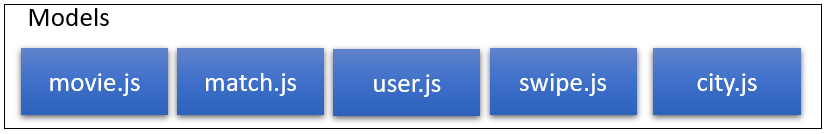
\includegraphics[width=8cm]{images/modelsstruktur.PNG}
\caption{NodeJSServer - Models Struktur}
\end{figure}

\paragraph{Datenzugriff}
Für den Datenzugriff auf die Datenbank wurden 


\begin{figure}[h]
\centering
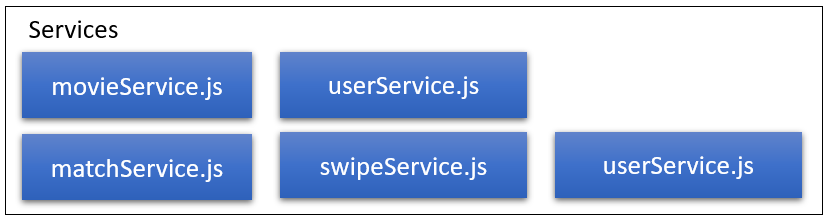
\includegraphics[width=8cm]{images/serviceStruktur.PNG}
\caption{NodeJSServer - Services Struktur}
\end{figure}